\documentclass{beamer}
\usepackage[utf8]{inputenc}
\usepackage[portuguese]{babel}
\usepackage{graphicx}
\usepackage{amsmath}
\usepackage{amssymb}
\usepackage{setspace} % Ajusta o espacamento entre linhas, em cada frame separamente.
\usepackage{hyperref} % Permite inserir links clicaveis.
\usepackage{subcaption}

\setbeamertemplate{caption}[numbered]

\hyphenpenalty=50
\tolerance=1000


% Escolha um tema (opcional, mas recomendável)
\usetheme{Madrid}  % Exemplo de tema


% Título, autor e outras informações (opcionais, mas recomendáveis)
\title{Programando com Arduino: do básico ao primeiro projeto}
\author{Laboratório Maker}
\institute{IFG - Câmpus Águas Lindas de Goiás}
\date{29 de Novembro de 2025}  % ou uma data fixa, ex: "27 de setembro de 2024"

\begin{document}

% Cria o slide de título
\begin{frame}
    \titlepage
\end{frame}

\begin{frame}{Introdução}
 
 \begin{columns}[T]  % [T] alinha o topo das colunas
    \begin{column}{0.55\textwidth}
        O \textbf{Arduino} é um \textcolor{blue}{microcontrolador programável de placa única}.
        \vspace{0.5cm}
        
        É um dispositivo que permite:
        \vspace{0.5cm}
        \begin{itemize}
         \item ler sinais do ambiente;
         \item controlar dispositivos eletrônicos de forma automática.
        \end{itemize}

        \vspace{0.5cm}
    
        O projeto do Arduino é de \textbf{hardware aberto}, ou seja:
        \vspace{0.5cm}
        \begin{itemize}
         \item o projeto é público e qualquer um pode copiar, estudar, modificar e fabricar placas compatíveis.
        \end{itemize}
        \vspace{0.5cm}
        

    \end{column}

    \begin{column}{0.45\textwidth}
        \begin{figure}
            \centering
            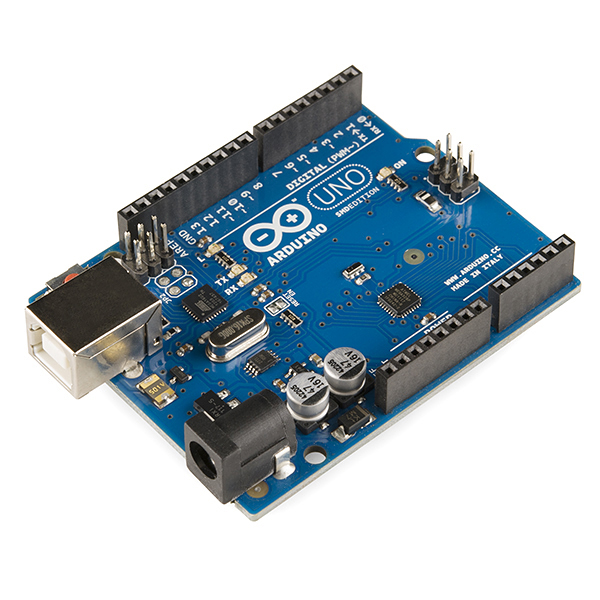
\includegraphics[width=\linewidth]{imagens/uno.jpg}
            \caption{Arduino Uno.}
        \end{figure}
    \end{column}
\end{columns}
 
\end{frame}

\begin{frame}{Aplicações}

\begin{columns}[T]  % [T] alinha o topo das colunas
    \begin{column}{0.55\textwidth}
    O Arduino possui diversas aplicações em sensoriamento e automação. 
    \vspace{0.5cm}


    Ao lado, temos a imagem de um sistema automatizado de \textbf{irrigação}.
    \vspace{0.5cm}
    
    O Arduino mede continuamente a umidade do solo e decide quando acionar ou desligar as bombas de irrigação.
    \vspace{0.5cm}
    
    
    Ele também envia esses dados para a internet, permitindo monitoramento remoto do sistema.

        

    \end{column}

    \begin{column}{0.45\textwidth}
        \begin{figure}
            \centering
            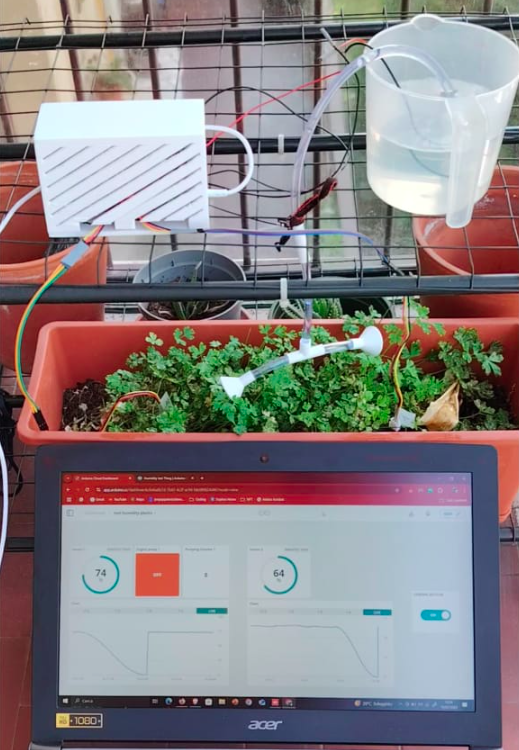
\includegraphics[width=0.7\linewidth]{imagens/planta.png}
            \caption{Sistema de irrigação automatizada.}
        \end{figure}
    \end{column}
\end{columns}

\end{frame}
 
 \begin{frame}{Aplicações}
 
 \begin{columns}[T]  % [T] alinha o topo das colunas
    \begin{column}{0.55\textwidth}
    Ao lado, temos outra aplicação. Um braço robótico de 6 graus de liberdade.
    \vspace{0.5cm}
 
    Ele manipula objetos pela combinação de:
    \begin{itemize}
        \item servomotores;
        \item estrutura metálica;
        \item controle eletrônico.
    \end{itemize}
    \vspace{0.5cm}

    O Arduino lê os comandos de posição dos potenciômetros e gera os sinais de controle para os servomotores, movimentando o braço.
        

    \end{column}

    \begin{column}{0.45\textwidth}
        \begin{figure}
            \centering
            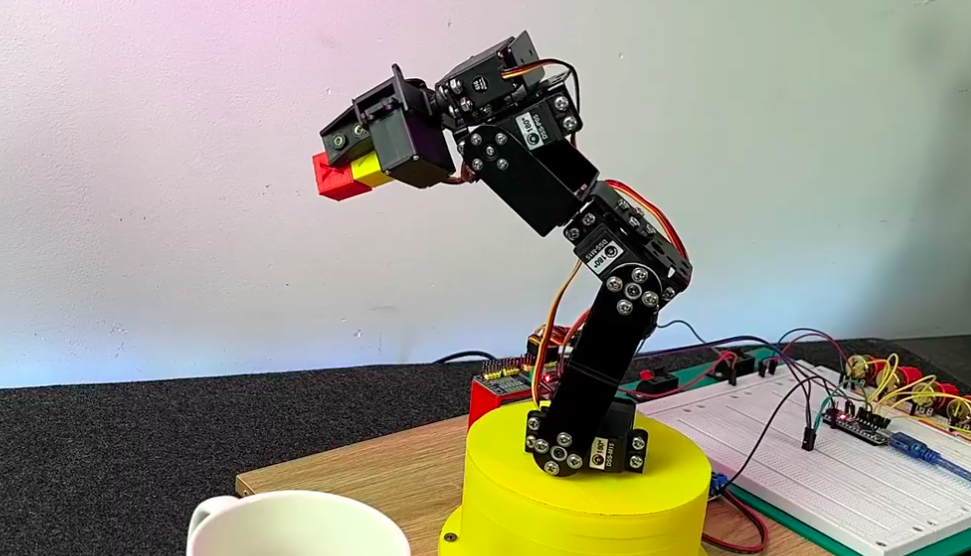
\includegraphics[width=\linewidth]{imagens/robo.png}
            \caption{Braço robótico.}
        \end{figure}
    \end{column}
\end{columns}
 
 
\end{frame}

\begin{frame}{Componentes}

  \begin{figure}
            \centering
            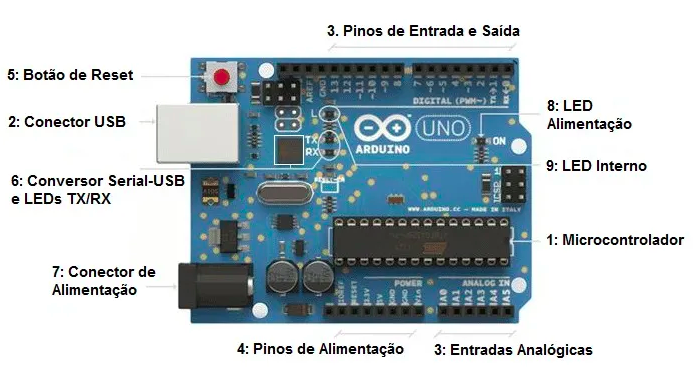
\includegraphics[width=\linewidth]{imagens/componentes.png}
            \caption{Componentes do Arduino Uno.}
        \end{figure}
 
 
\end{frame}

\begin{frame}{Componentes}
 
 1 - Microcontrolador
 \begin{itemize}
  \item É aqui que o seu código é armazenado e executado. Pense nele como o processador de um computador, mas focado em controlar tarefas simples (como ler um sensor ou acender uma luz).
 
 \end{itemize}
\vspace{0.5cm}

2 - Conector USB

\begin{itemize}
 \item Função: Serve para conectar o Arduino ao seu computador.
 \item Utilidade: É através dele que você envia (carrega) o código que escreveu no computador para a placa. Ele também fornece energia para ligar o Arduino (5 Volts).
\end{itemize}




 
\end{frame}

\begin{frame}{Componentes}
 
 3 - Pinos de entrada e saída
\begin{itemize}
 \item \textbf{Parte Superior (Digital):} São os pinos digitais (numerados de 0 a 13). Eles podem ligar/desligar coisas (como LEDs) ou ler estados simples (botão pressionado ou solto). Alguns têm um $\sim$ ao lado, indicando que podem simular sinais analógicos (PWM).
 \begin{figure}
            \centering
            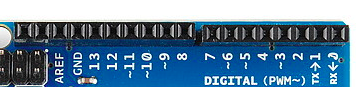
\includegraphics[width=0.7\linewidth]{imagens/pinos_digitais.png}
%             \caption{Sistema de irrigação automatizada.}
        \end{figure}
 
 \item \textbf{Parte Inferior Direita (Analógicas):} Identificados como A0 a A5. Estes pinos "leem" voltagens variáveis. São usados para sensores que não são apenas "ligado/desligado", como um sensor de temperatura ou de luminosidade.
 
  \begin{figure}
            \centering
            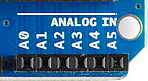
\includegraphics[width=0.3\linewidth]{imagens/pino_analogico.png}
%             \caption{Sistema de irrigação automatizada.}
        \end{figure}
\end{itemize}
 
 
\end{frame}

\begin{frame}{Componentes}
 
4 - Pinos de Alimentação (Power) 
  \begin{figure}
            \centering
            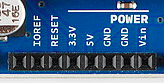
\includegraphics[width=0.3\linewidth]{imagens/pino_alimentacao.png}
%             \caption{Sistema de irrigação automatizada.}
        \end{figure}

\begin{itemize}
 \item Esta área fornece energia para componentes externos que você conectar ao Arduino.
 \item Detalhes:
 \begin{itemize}
    \item \textbf{3.3V e 5V}: Fornecem voltagem constante para sensores.
    \item \textbf{GND}: O "Terra" ou negativo (essencial para fechar o circuito).
    \item \textbf{VIN}: Entrada de voltagem (se você quiser alimentar o Arduino por aqui em vez do conector preto).
    \item \textbf{RES (RESET)}: Permite resetar o Arduino ao conectá-lo com um pino GND.
 \end{itemize}
\end{itemize}

 
 
\end{frame}

\begin{frame}{Componentes}
 
 5 - Botão de Reset
  \begin{figure}
            \centering
            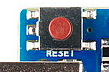
\includegraphics[width=0.3\linewidth]{imagens/reset.png}
%             \caption{Sistema de irrigação automatizada.}
        \end{figure}
 \begin{itemize}
  \item Ao ser pressionado, ele interrompe o que o Arduino está fazendo e reinicia o código do zero.
  \item Útil se o seu programa travar ou se você quiser ver o código rodar desde o início novamente.
 \end{itemize}
\vspace{0.5cm}


 
\end{frame}

\begin{frame}{Componentes}
\begin{columns}[T]
    \begin{column}{0.55\textwidth}
    
    6 - Conversor Serial-USB e LEDs TX/RX 
    \begin{itemize}
     \item \textbf{Conversor:} É um pequeno chip auxiliar que traduz a linguagem do USB (do computador) para a linguagem Serial (que o Microcontrolador principal entende).
     \item \textbf{LEDs TX (Transmitir) e RX (Receber)}: Essas pequenas luzes piscam rapidamente quando o Arduino está trocando dados com o computador (por exemplo, enquanto você está enviando um código novo).
    \end{itemize}

      \textbf{Obs.:} Na placa de vocês, o TX está abaixo do RX, de cabeça para baixo.   

    \end{column}

    \begin{column}{0.45\textwidth}
        \begin{figure}
            \centering
            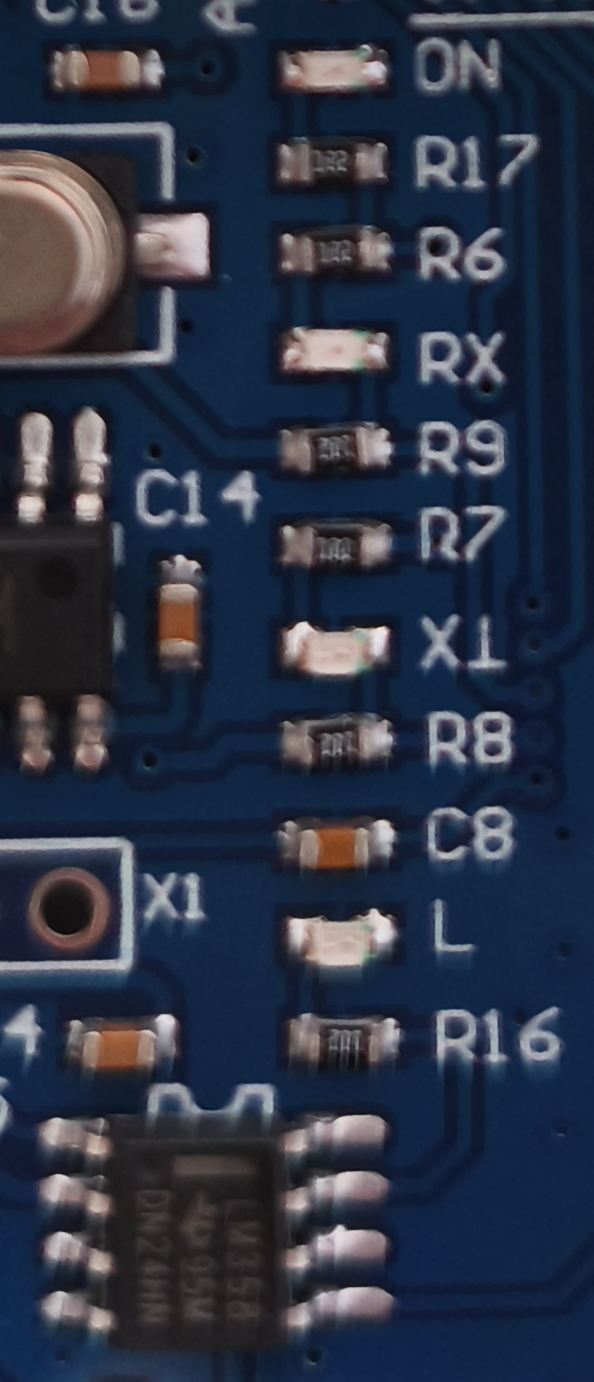
\includegraphics[width=0.4\linewidth]{imagens/rx_tx.jpg}
%             \caption{Braço robótico.}
        \end{figure}
    \end{column}
\end{columns}
        
 


\end{frame}

\begin{frame}{Componentes}
 
 7 - Conector de Alimentação (Jack P4)
 
   \begin{figure}
            \centering
            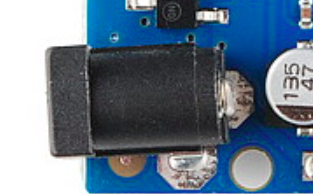
\includegraphics[width=0.3\linewidth]{imagens/jack.png}
%             \caption{Sistema de irrigação automatizada.}
        \end{figure}
        
    \begin{itemize}
     \item Permite ligar o Arduino sem precisar do computador.
     \item Você pode conectar uma bateria de 9V ou uma fonte de tomada (geralmente entre 7V e 12V) aqui para que seu projeto funcione de forma autônoma.
    \end{itemize}

 
 
\end{frame}

\begin{frame}{Componentes}
 


\begin{columns}[T]  % [T] alinha o topo das colunas
    \begin{column}{0.55\textwidth}
    
    8 - LED Alimentação (ON)
    \begin{itemize}
     \item Função: Uma luz verde simples que acende assim que a placa recebe energia.
     \item Diagnóstico: Se você ligar o Arduino e essa luz não acender, algo está errado com a fonte de energia.
    \end{itemize}

        

    \end{column}

    \begin{column}{0.45\textwidth}
        \begin{figure}
            \centering
            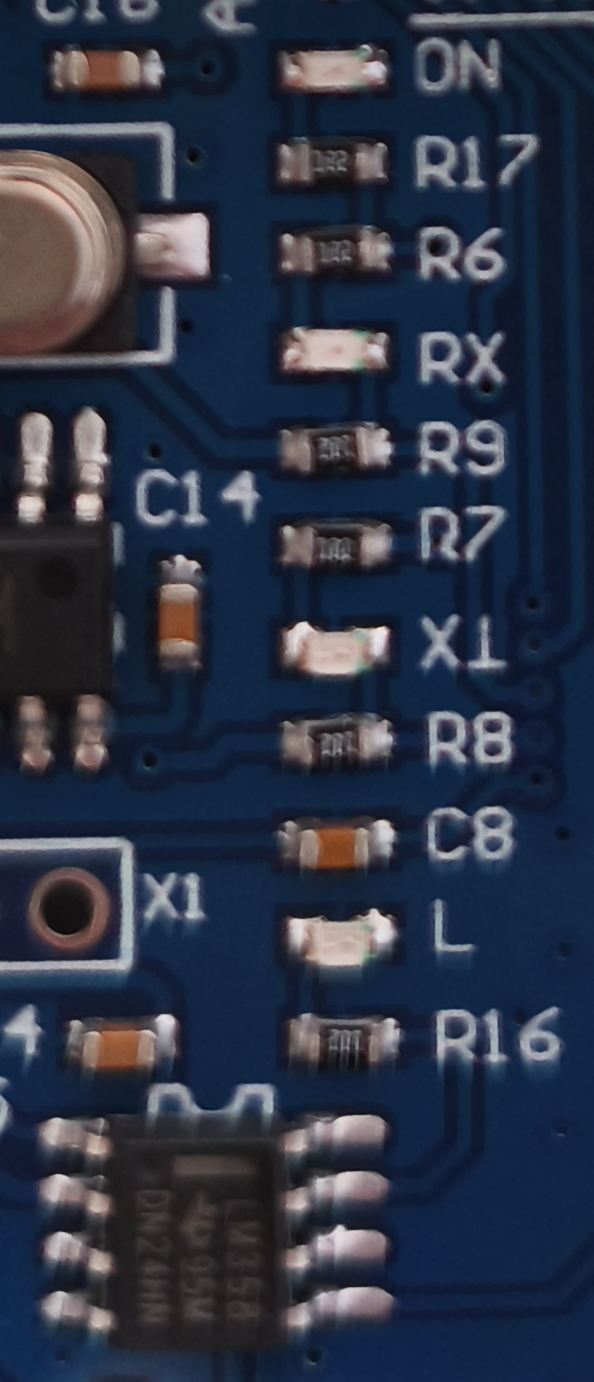
\includegraphics[width=0.4\linewidth]{imagens/rx_tx.jpg}
%             \caption{Braço robótico.}
        \end{figure}
    \end{column}
\end{columns}
        
 
\end{frame}

\begin{frame}{Componentes}
 
 






\begin{columns}[T]  % [T] alinha o topo das colunas
    \begin{column}{0.55\textwidth}
    
    9 - LED Interno (L)
\begin{itemize}
 \item Função: Um LED laranja já embutido na placa para testes rápidos.
 \item Conexão: Ele está conectado internamente ao Pino Digital 13. Isso é ótimo para testar se a placa está funcionando (o famoso código "Blink") sem precisar montar circuitos externos.
\end{itemize}

        

    \end{column}

    \begin{column}{0.45\textwidth}
        \begin{figure}
            \centering
            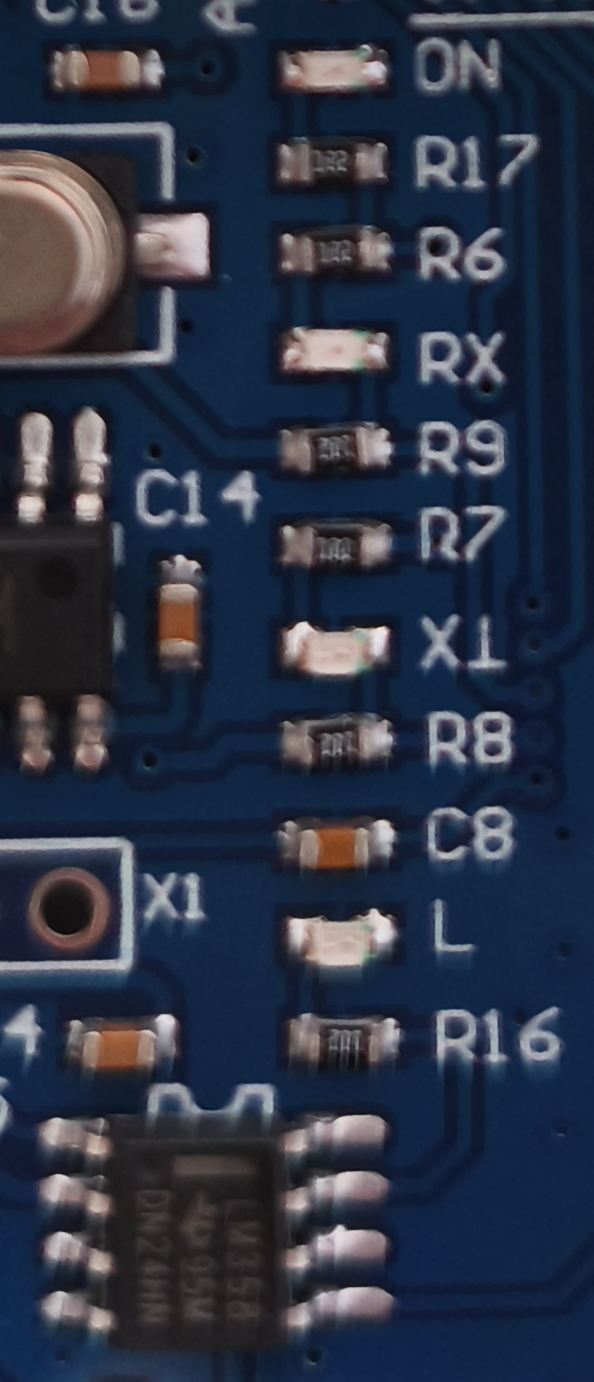
\includegraphics[width=0.4\linewidth]{imagens/rx_tx.jpg}
%             \caption{Braço robótico.}
        \end{figure}
    \end{column}
\end{columns}
 
 
\end{frame}

\begin{frame}{Programação}
 
 
 O Arduino contém um microcontrolador programável, o que significa que é preciso criar um \textbf{programa} que dirá o que ele deve fazer.
 \vspace{0.5cm}
 
 Programa-se um Arduino escrevendo um \textbf{código} (chamado \textcolor{blue}{“sketch”}) em uma linguagem baseada em C/C++ dentro do \textcolor{red}{Arduino IDE} (um programa de computador) ou ambiente compatível.
 \vspace{0.5cm}
 
 No \textcolor{red}{Tinkercad Circuits} (um site de programação), a programação em blocos é uma forma visual de programar o Arduino sem escrever código em C/C++, usando \textbf{blocos encaixáveis}.
 \vspace{0.5cm}
 
 A seguir, vamos aprender a programar um Arduino com alguns projetos simples.
 
\end{frame}



\end{document}
